% Template for a Computer Science Tripos Part II project dissertation
\documentclass[12pt,a4paper,twoside,openright]{report}

\usepackage{My_style}
\usepackage{dirtree}
\usepackage{minted}
\usepackage[pdfborder={0 0 0}]{hyperref}    % turns references into hyperlinks
\usepackage[margin=25mm]{geometry}  % adjusts page layout
\usepackage{graphicx}  % allows inclusion of PDF, PNG and JPG images
\usepackage{verbatim}
\usepackage{docmute}   % only needed to allow inclusion of proposal.tex
\usepackage[utf8]{inputenc}
\usepackage{mathtools}
\usepackage{changepage}
\usepackage{url}
\usepackage{stmaryrd}
\usepackage{blindtext}
\usepackage{epigraph}
\usepackage{amssymb}

\usepackage{newunicodechar}
\usepackage{ifthen}

\newunicodechar{ℕ}{\ensuremath{\mathnormal {\mathbb{N}}}}
\newunicodechar{𝔹}{\ensuremath{\mathnormal {\mathbb{B}}}}
\newunicodechar{→}{\ensuremath{\mathnormal {\to}}}

\newunicodechar{⌞}{\ensuremath{\llcorner}}
\newunicodechar{⌟}{\ensuremath{\lrcorner}}
\newunicodechar{′}{\ensuremath{\prime}}
\newunicodechar{−}{\ensuremath{-}}
\newunicodechar{─}{\ensuremath{-}}
\newunicodechar{—}{\ensuremath{--}}
\newunicodechar{◆}{\ensuremath{\Diamondblack}}
\newunicodechar{⧫}{\ensuremath{\blacklozenge}}
\newunicodechar{∷}{\ensuremath{::}}
\newunicodechar{∙}{\ensuremath{\bullet}}
\newunicodechar{□}{\ensuremath{\Box}}
\newunicodechar{∎}{\ensuremath{\blacksquare}}
\newunicodechar{⋆}{\ensuremath{\star}}
\newunicodechar{●}{\scalebox{0.8}{$\bullet$}}
\newunicodechar{▸}{{\scalebox{0.7}{$\blacktriangleright$}}}


% indices
\newunicodechar{₀}{\ensuremath{_0}}
\newunicodechar{₁}{\ensuremath{_1}}
\newunicodechar{₂}{\ensuremath{_2}}
\newunicodechar{₃}{\ensuremath{_3}}

\newunicodechar{ₚ}{\ensuremath{_*}}
\newunicodechar{ₑ}{\ensuremath{_e}}
\newunicodechar{ᵢ}{\ensuremath{_i}}
\newunicodechar{ₖ}{\ensuremath{_k}}
\newunicodechar{ₘ}{\ensuremath{_m}}
\newunicodechar{ₙ}{\ensuremath{_n}}
\newunicodechar{ᵣ}{\ensuremath{_r}}
\newunicodechar{ₛ}{\ensuremath{_{\scriptscriptstyle \mathrm{S}}}}
\newunicodechar{ₓ}{\ensuremath{_X}}
\newunicodechar{ₗ}{\ensuremath{_l}}

\newunicodechar{₊}{\ensuremath{_+}}

% exponents
\newunicodechar{⁺}{\ensuremath{\textsuperscript{+}}}
\newunicodechar{⁻}{\ensuremath{\textsuperscript{-}}}

\newunicodechar{²}{\ensuremath{^2}}

\newunicodechar{ⁱ}{\ensuremath{^i}}


% ticks
\newunicodechar{′}{\ensuremath{'}}
\newunicodechar{″}{\ensuremath{'}}
% \newunicodechar{ˡ}{\ensuremath{^l}}
\newunicodechar{ᵐ}{\ensuremath{^{\scriptscriptstyle\mathrm{M}}}}
\newunicodechar{ʳ}{\ensuremath{^r}}
\newunicodechar{ᵒ}{\ensuremath{^o}}
\newunicodechar{ˢ}{\ensuremath{^s}}
\newunicodechar{ᶠ}{\ensuremath{^f}}
\newunicodechar{ᶜ}{\textsuperscript{c}}
\newunicodechar{ᵇ}{\ensuremath{^{\scriptscriptstyle\bo}}}
\newunicodechar{ᴮ}{\ensuremath{_*^{\scriptscriptstyle\bo}}}

\newunicodechar{ᴬ}{\ensuremath{^A}}
\newunicodechar{ᴵ}{\ensuremath{^I}}
\newunicodechar{ᴿ}{\ensuremath{^R}}
\newunicodechar{ᵀ}{\ensuremath{^T}}
\newunicodechar{ᵁ}{\ensuremath{^U}}
\newunicodechar{ⱽ}{\ensuremath{^V}}
\newunicodechar{ˡ}{\ensuremath{^{\scriptscriptstyle\Sigma}}}
\newunicodechar{ᴸ}{\ensuremath{^L}}
\newunicodechar{ᴹ}{\ensuremath{^{\scriptscriptstyle\mathrm{M}}}}


% Dots
\newunicodechar{⋯}{\ensuremath{\cdots}}

% Equality symbols
\newunicodechar{≡}{\ensuremath{\equiv}}
\newunicodechar{≢}{\ensuremath{\not\equiv}}
\newunicodechar{≟}{\mbox{\tiny\ensuremath{\stackrel{?}{=}}}}
\newunicodechar{≈}{\ensuremath{\approx}}

% Ordering symbols
\newunicodechar{≼}{\ensuremath{\preccurlyeq}}
\newunicodechar{≤}{\ensuremath{\le}}
\newunicodechar{⊑}{\ensuremath{\sqsubseteq}}
\newunicodechar{≥}{\ensuremath{\ge}}

% Arrows
\newunicodechar{→}{\ensuremath{\rightarrow}}
\newunicodechar{←}{\ensuremath{\leftarrow}}
\newunicodechar{⇒}{\ensuremath{\scriptstyle\Rightarrow}}
\newunicodechar{⇉}{\ensuremath{\rightrightarrows}}
\newunicodechar{↣}{\ensuremath{\funty}}
\newunicodechar{↝}{\ensuremath{\ren}}
\newcommand{\hackctxmap}[2]{\ctxmap{#1}}
\newunicodechar{⇝}{\hackctxmap}
\newunicodechar{⟶}{\ensuremath{\rightarrow}}
\newunicodechar{↦}{\ensuremath{\mapsto}}
\newunicodechar{↻}{\ensuremath{\circlearrowleft}}
\newunicodechar{⟿}{\ensuremath{\rightsquigarrow}}
\newunicodechar{◅}{\ensuremath{\triangleleft}}

% Mathematical symbols
\newunicodechar{∂}{\ensuremath{\partial}}
\newunicodechar{∋}{\ensuremath{\ni}}
\newunicodechar{∞}{\ensuremath{\infty}}
\newunicodechar{∀}{\ensuremath{\forall}}
\newunicodechar{∃}{\ensuremath{\exists}}
\newunicodechar{∄}{\ensuremath{\nexists}}
\newunicodechar{⊢}{\ensuremath{\vdash}}
\newunicodechar{⟨}{\ensuremath{\langle}}
\newunicodechar{⟩}{\ensuremath{\rangle}}
\newunicodechar{⊤}{\ensuremath{\top}}
\newunicodechar{∘}{\ensuremath{\circ}}
\newunicodechar{⊎}{\ensuremath{\uplus}}
\newunicodechar{×}{\ensuremath{\times}}
\newunicodechar{ℕ}{\ensuremath{\mathbb{N}}}
\newunicodechar{⟦}{\ensuremath{\llbracket}}
\newunicodechar{⟧}{\ensuremath{\rrbracket}}
\newunicodechar{∈}{\ensuremath{\in}}
\newunicodechar{↑}{\ensuremath{\uparrow}}
\newunicodechar{¬}{\ensuremath{\neg}}
\newunicodechar{⊥}{\ensuremath{\bot}}
\newunicodechar{↝}{\ensuremath{\leadsto}}
\newunicodechar{↶}{\ensuremath{\curvearrowleft}}
\newunicodechar{↺}{\ensuremath{\circlearrowleft}}
\newunicodechar{⊔}{\ensuremath{\sqcup}}
\newunicodechar{⨆}{\ensuremath{\bigsqcup}}
\newunicodechar{⋃}{\ensuremath{\bigcup}}
\newunicodechar{∩}{\ensuremath{\cap}}
\newunicodechar{∪}{\ensuremath{\cup}}
\newunicodechar{∅}{\ensuremath{\emptyset}}
\newunicodechar{∙}{\ensuremath{\cdot}}
\newunicodechar{∔}{\ensuremath{\app}}
\newunicodechar{⊗}{\ensuremath{\otimes}}
\newunicodechar{⊕}{\ensuremath{\oplus}}
\newunicodechar{⊖}{\ensuremath{\ominus}}
\newunicodechar{⊙}{\ensuremath{\FTens}}
\newunicodechar{⊸}{\ensuremath{\linto}}
\newunicodechar{⇾}{\ensuremath{\famto}}
\newunicodechar{⇨}{\ensuremath{\Rightarrow}}
\newunicodechar{′}{\ensuremath{'}}
\newunicodechar{〖}{\ensuremath{{\lwbrak}}}
\newunicodechar{〗}{\ensuremath{{\rwbrak}}}


% Misc
\newunicodechar{ℓ}{\ensuremath{\ell}}

% Greek uppercase
\newunicodechar{Δ}{\ensuremath{\Delta}}
\newunicodechar{Γ}{\ensuremath{\Gamma}}
\newunicodechar{Λ}{\ensuremath{\Lambda}}
\newunicodechar{Σ}{\ensuremath{\Sigma}}
\newunicodechar{Θ}{\ensuremath{\Theta}}
\newunicodechar{Ξ}{\ensuremath{\Xi}}
\newunicodechar{Ω}{\ensuremath{\Omega}}

% Greek lowercase
\newunicodechar{α}{\ensuremath{\alpha}}
\newunicodechar{β}{\ensuremath{\beta}}
\newunicodechar{δ}{\ensuremath{\delta}}
\newunicodechar{ε}{\ensuremath{\epsilon}}
\newunicodechar{φ}{\ensuremath{\phi}}
\newunicodechar{ϕ}{\ensuremath{\varphi}}
\newunicodechar{γ}{\ensuremath{\gamma}}
\newunicodechar{ι}{\ensuremath{\iota}}
\newunicodechar{κ}{\ensuremath{\kappa}}
\newunicodechar{λ}{\ensuremath{\lambda}}
\newunicodechar{μ}{\ensuremath{\mu}}
\newunicodechar{ψ}{\ensuremath{\psi}}
\newunicodechar{η}{\ensuremath{\eta}}
\newunicodechar{ρ}{\ensuremath{\rho}}
\newunicodechar{ϱ}{\ensuremath{\varrho}}
\newunicodechar{σ}{\ensuremath{\sigma}}
\newunicodechar{ς}{\ensuremath{\varsigma}}
\newunicodechar{τ}{\ensuremath{\tau}}
\newunicodechar{ξ}{\ensuremath{\xi}}
\newunicodechar{χ}{\ensuremath{\chi}}
\newunicodechar{ζ}{\ensuremath{\zeta}}
\newunicodechar{Π}{\ensuremath{\Pi}}
\newunicodechar{ω}{\ensuremath{\omega}}
\newunicodechar{ƛ}{\ensuremath{\boldsymbol{\lambda}}}

\newunicodechar{ℐ}{\ensuremath{\Ind}}

% Macros

\newcommand{\agdacode}[2][CoreL]{\begin{spacing}{1.1}%
\ExecuteMetaData[formalisation/agda/latex/#1.tex]{#2}%
\end{spacing}}
\newcommand{\aty}[2]{\AgdaBound{#1}\,\AgdaSymbol{:}\,\AgdaDatatype{#2}}

\newcommand{\Actxmap}[3]{#1\AgdaSpace{}%
\AgdaOperator{\AgdaFunction{–[}}\AgdaSpace{}%
\AgdaBound{#2}\AgdaSpace{}%
\AgdaOperator{\AgdaFunction{]→}}\AgdaSpace{}%
#3}



%%%%%%%%%% AGDA ALIASES

\newcommand{\APT}{\AgdaPrimitiveType}
\newcommand{\AK}{\AgdaKeyword}
\newcommand{\AM}{\AgdaModule}
\newcommand{\AS}{\AgdaSymbol}
\newcommand{\AStr}{\AgdaString}
\newcommand{\AN}{\AgdaNumber}
\newcommand{\AD}{\AgdaDatatype}
\newcommand{\AF}{\AgdaFunction}
\newcommand{\AR}{\AgdaRecord}
\newcommand{\ARF}{\AgdaField}
\newcommand{\AB}{\AgdaBound}
\newcommand{\AIC}{\AgdaInductiveConstructor}
\newcommand{\AO}{\AgdaOperator}
\newcommand{\AUS}{\AgdaUnderscore{}}
\newcommand{\AG}{\AgdaGeneralizable}
\newcommand{\AAr}{\AgdaArgument}
\newcommand{\AInd}{\AgdaIndent}


%\raggedbottom                           % try to avoid widows and orphans
\sloppy
\clubpenalty1000%
\widowpenalty1000%

\renewcommand{\baselinestretch}{1.1}    % adjust line spacing to make
                                        % more readable

\begin{document}


\newcommand{\mcandidate}{UNCLEAR}
\newcommand{\mfullname}{Patrick Nickols}
\newcommand{\mcollege}{Downing College}
\newcommand{\mtitle}{Formalising PCF and its Denotational Semantics in Agda}
\newcommand{\mexamination}{Computer Science Tripos -- Part II}
\newcommand{\mdate}{TBD}
\newcommand{\moriginator}{Mr Dima Szamozvancev}
\newcommand{\msupervisor}{Mr Dima Szamozvancev}
\newcommand{\mwordcount}{TBD}
\newcommand{\mlinecount}{TBD}
% Consent to the dissertation made available to University members
\newcommand{\mconsent}{I am content for my dissertation to be made available to the students and staff of the University.}
% For the Declaration of originality
\newcommand{\msignature}{Patrick David Nickols}

\bibliographystyle{plain}


%%%%%%%%%%%%%%%%%%%%%%%%%%%%%%%%%%%%%%%%%%%%%%%%%%%%%%%%%%%%%%%%%%%%%%%%
% Title


\thispagestyle{empty}

\rightline{\LARGE \textbf{\mfullname}}

\vspace*{60mm}
\begin{center}
\Huge
\textbf{\mtitle} \\[5mm]
\mexamination \\[5mm]
\mcollege \\[5mm]
\mdate  % today's date
\end{center}

%%%%%%%%%%%%%%%%%%%%%%%%%%%%%%%%%%%%%%%%%%%%%%%%%%%%%%%%%%%%%%%%%%%%%%%%%%%%%%
% Proforma, table of contents and list of figures

\pagestyle{plain}

\newpage
\newpage
\section*{Declaration of originality}

I, \mfullname{} of \mcollege, being a candidate for Part II of the Computer Science Tripos, hereby declare that this dissertation and the work described in it are my own work, unaided except as may be specified below, and that the dissertation does not contain material that has already been used to any substantial extent for a comparable purpose. \mconsent

\bigskip
\leftline{Signed \msignature}
\bigskip
\leftline{Date \today}

\chapter*{Proforma}

{\large
\begin{tabular}{ll}
Candidate Number:   & \bf \mcandidate                   \\
Project Title:      & \bf \mtitle                       \\
Examination:        & \bf \mexamination, \mdate         \\
Word Count:         & \bf \mwordcount\footnotemark[1]   \\
Code Line Count:    & \bf \mlinecount                   \\
Project Originator: & \bf \moriginator                  \\
Supervisor:         & \bf \msupervisor                  \\ 
\end{tabular}
}
\footnotetext[1]{This word count was computed
by \texttt{detex diss.tex | tr -cd '0-9A-Za-z $\tt\backslash$n' | wc -w}
}
\stepcounter{footnote}


\section*{Original Aims of the Project}
% At most 100 words

TODO


\section*{Work Completed}
% At most 100 words

TODO

\section*{Special Difficulties}
% At most 100 words

TODO

\newpage

\tableofcontents

\listoffigures

\newpage
\section*{Acknowledgements}

TODO

%%%%%%%%%%%%%%%%%%%%%%%%%%%%%%%%%%%%%%%%%%%%%%%%%%%%%%%%%%%%%%%%%%%%%%%
% now for the chapters

\pagestyle{headings}

\chapter{Introduction}
\section{Motivation}
\epigraph{Beware of bugs in the above code; I have only proved it correct, not tried it.}{--- \textup{Donald Knuth}}

Everyone who writes code frequently has written buggy code. The costs of these errors vary from minor decreases of self-esteem on the behalf of the programmer to large financial losses (CITE HERE) and, in some cases, deaths (CITE HERE). Programmers have year after year been flummoxed by increasingly unpredictable errors, as programs grow too complicated to easily reason about, but too useful to discard. Various approaches have been suggested to deal with this, and one calling out from those with a mathematical background is formalisation - defining precisely what it is that programs can and should do. This specification of the ``meaning" of a language and its programs is called ``semantics"\footnote{This term comes to the computer science community from linguistics, where its meaning is similar. The study of the semantics of a spoken language is the study of its words and sentences' meanings.}. 

While this seems an attractive idea, there are clear problems with backpatching formalisation onto existing languages. C, whose applications power most of the modern technological world, \textit{does not have a formal semantics}, while producing a parse tree for C++ \textit{is undecidable}, which implies its semantics are severely underspecified(CITES). 

The challenge then, is finding a middle ground between useless formalisation of unimportant concepts in impractical languages, and the impossibility of formalising the most relevant concepts in the most relevant languages. 

\section{Background}
\subsection{(Denotational) Semantics}
After one decides it's worth trying to formalise what a language means and what its programs do, there are several approaches, which are generally said to fall into one of three categories (Footnote about who agrees there are 3 main ones).

\textit{Axiomatic Semantics} reasons in terms of precondition and postconditions: assertions that are true before some code is run and the corresponding assertions that must be true after accordingly.

\textit{Operational Semantics} describes how programs transform as they are run in terms of a reduction relation\footnote{With deterministic small-step reduction, we hope that the reduction relation is a function, i.e. that each term reduces in at most one way.} saying that e.g. \texttt{if true then x else y} reduces to \texttt{x}. This approach is to some extent implictly required by anyone creating a programming language. While it may not be formalised and precise, to invent a programming language, one needs to impart meaning to its keywords, and thus have a mental model of what each operation does. 

\textit{Denotational Semantics} aims to find a correspondence between programs and mathematical objects, with the hope being that one can reason about the objects more easily, using tools from mathematics. Ideally the correspondence is meaningful in mathematically provable ways\footnote{For example, we hope if that if a term reduces via the operational semantics to another term, their denotations are related in some way (in fact, we normally want equality between the two terms). This property is called soundness and is detailed more later.}. It is this approach that I will be following. 

While this may sound abstract, I claim that in certain cases this is obvious and even done implicitly: the common mental model for a programming language's integer type is the set $\mathbb{Z}$\footnote{In reality, many languages don't support arbitrary integers in their int type, but a restricted class. In this case the mental model may be a subset of $\mathbb{Z}$.}. The question in this case becomes what to do when things are not obvious, or the obvious thing fails? We can view product types as corresponding to (cartesian) products of sets, and functions to functions, but what then does \texttt{while} correspond to? And how do we know that our chosen interpretation is effective and useful? These are the sorts of questions that the denotational semantics course aims to answer. One level higher, the course's answers are the questions that my dissertation aims to formalise. 
\subsection{PCF}
Programming Computable Functions, (from here on PCF), is a toy programming language created by Dana Scott (CITE) for the express purpose of defining a denotational semantics. It is thus small, but sufficiently non-trivial that defining its semantics could yield a publishable paper\footnote{In fact, the cognoscenti will note that this skims over some important details. The paper was not concerned with a programming language PCF, but merely a logical system (which Scott called LCF). Scott was seeking an alternative to the lambda calculus as a model of computation. It was extended to a programming language in (?) by Plotkin (CITE)}. Slightly different versions of it exist in the literature; I will use the modern \footnote{In particular, Scott avoided lambdas (he thought substitution theorems were a pain!), and had K and S combinators instead.} one (almost exactly) as defined in the course. While we later get to its precise terms and types (Where?), it is a good approximation to think of it as a variant on the simply-typed lambda calculus, with ground types of booleans and integers, and the basic corresponding operations (if-expressions, a test-for-zero, the successor and predecessor functions). 

The defining feature of PCF, which leads directly to the denotational objects chosen to represent its terms is the fixpoint operator. Given a function $f : A \to A$, we have $\text{fix}(f) = f (\text{fix}(f))$ (where $=$ is being used approximately). That is the fixpoint of $f$ is an input to $f$ whose output is itself, i.e. a fixed point of $f$. From a practical point of view, this allows us to implement recursion: e.g. to define $f(n) = n!$ we can write\footnote{in an approximate notation, the details of language syntax are not the point here.}
\[
\text{fix}\left( \lambda f : \text{nat} \to \text{nat}. \lambda n: \text{nat}. \text{if } n = 0 \text{ then } 1 \text{ else } n * f (n-1)\right).
\] This is analogous to the $Y$-combinator of the untyped lambda calculus. However, the untyped lambda calculus is a pathological language, where any term can be an input to any function\footnote{Scott wrote that the untyped lambda calculus ``makes no sense whatsoever".} and every function has a fixed point. It is thus perhaps surprising that in PCF, where we have types and slightly ``better behaviour", we still expect every function to have a fixpoint. What, one may ask, should the fixpoint of the successor function be, given that clearly we don't have any $n$ such that $n+1 = n$? 

It is exactly this question: ``what mathematical objects guarantee us that all functions have fixed points?" that led Scott to his chosen semantics of domains and continuous functions\footnote{In fact, the avid historian may take issue with this characterisation. Scott's paper discusses the difficulties of simulating partial functions with total functions, and says that stumbling upon domains was mainly a consequence of trying to represent undefined behaviour with the extra element $\bot$. That everything ends up working out so nicely with the fixed point operator he attributes to luck.}.

 

\section{Project Description}
The aim of the project was to formalise the main results of the Denotational Semantics course. In particular, from the first half of the course, I wanted to formalise:
\begin{itemize}
\item Lambek's Lemma (that the least pre-fixed point is itself a fixed point)
\item Tarski's fixed point theorem
\item The continuity of the fixpoint operator.
\end{itemize}
And from the second part of the course, concerning PCF and its denotation, I wanted to formalise:
\begin{itemize}
\item The language PCF itself
\item Its denotational semantics
\item A progress theorem (that well-typed terms don't get stuck, they are either values or can reduce)
\item A preservation theorem (that terms have the same type before and after reduction)
\item A soundness theorem for its semantics (that if one term reduces to another, then they have the same denotation).
\end{itemize}
Extensions that I considered at the time of proposing were:
\begin{itemize}
\item A category-theoretic perspective on the same material
\item A compositionality theorem (that if two terms have the same denotation, all contexts with one swapped for the other also have the same denotation)
\item An adequacy theorem (that for ground-typed terms, if they have the same denotation, one reduces to the other). 
\item Scott induction (a specific induction principle when dealing with the fixed point operator). 
\end{itemize}
Of these, I tackled the second and fourth (haven't actually done yet).
\section{Related Work}
The most relevant work being produced in the last few years has come primarily from the UK, notably the research group of Birmingham, involving work by Escardo, De Jong, and Hart. However, their work, while attacking the same or similar problems (also in Agda), answers these questions via the lens of Homotopy Type Theory. This is an abstract approach primarily motivated by Voevodsky, that has been working to reshape mathematics' underpinnings, avoiding ZFC as a foundational model, and instead aiming at type-theoretic primitives\footnote{This effort primarily intensified between 2012 and 2013, when the Institute for Advanced Study held ``A special year on Univalent Foundations in Mathematics": a year dedicated to advancing and propogating the spread of this thinking.}. I will not dwell too much on its details but the curious reader is invited to (CITE), but note that this approach is different in motivation and direction from my project\footnote{In particular, ???}, though we prove some of the same theorems.
Beyond that, Streicher covers much of the material at (CITE), but with a pen-and-paper approach while Wadler (CITE) covers using Agda as a proof assistant, and implementing a PCF-like language, but does not implement its denotational semantics\footnote{He instead implements a denotational semantics for the untyped lambda calculus.}. Finally I am indebted to (CITE), as an example of how to write a Cambridge Part II Dissertation with an Agda project: although we proved quite different things, there are heavy motivational overlaps. 
\chapter{Preparation}
\section{PCF}
\subsection{Syntax}
The variant of PCF we will be considering looks much like a simply-typed lambda calculus with a few ground terms and primitives, and the key extra feature of a fixpoint operator. Its grammar is defined by (where $\mu$ is the fixpoint operator and $x$ is a fresh variable name\footnote{Although, since we will use de Bruijn indices, this is just a visual aid.}):
\[
L, M, N := x \mid \text{Zero} \mid \text{True} \mid \text{False} \mid \lambda x: \tau . M \mid M \cdot N 
\]
\[
\text{Succ }M \mid \text{Pred }M \mid \text{Is-Zero }M \mid \text{If }L \text{ then }M \text{ else }N \mid \mu M
\]
\subsection{Typing Relation}
The typing relation is unsurprising. We have a type of naturals, a type of booleans, and function types. Note in particular that because of design decisions in implementation, we will only deal with well-typed terms.
\subsection{Notable Features}
PCF is Turing complete. This is a well-known result, and its proof is expressed in the lecture notes. It relies upon the lemma that partial recursive functions are Turing-complete. We then show that we can encode partial recursion in PCF, and are thus done. The key details are that we have natural numbers, the fixpoint operator and case-destructors for integers - equivalent forms of PCF have a case matching on integers with $0$ and suc($n$) that suffices as well\footnote{C.f. e.g. CITE}. 

A perhaps surprising result is that the fixpoint operator (which allows unbounded recursion) is not sufficient on its own: in the simply typed lambda calculus augmented with only the Y combinator, everything, in particular whether a program terminates, is decidable. Details can be found in Statman's (CITE). 
\subsection{Relation to other languages}
A natural question to ask, and a common refrain from those who work on more applied subjects is something along the lines of ``What's the point? Are you really proving anything if you only deal with toy languages?". However these concerns can be addressed in two ways. Firstly, it should be noted that progress is incremental: it was easier to give an operational semantics for languages that closely model the typed lambda calculus than for C, but seeing an operational semantics for the typed lambda calculus makes providing one for C much more feasible. 

Secondly, and of some importance for the PCF-interested reader: PCF was the inspiration behind ML and thus OCaml, F\# etc. In particular, Milner developed ML for a theorem-proving system based on LCF. Proving things about PCF can thus be viewed as foundational work for proving things about languages like OCaml, Haskell and F\#.
\section{Agda}
\subsection{Curry--Howard}
The Curry--Howard correspondence is undoubtedly one of the most intriguing connections between logic and computer science. While it may not seem surprising that product types correspond to conjunctions, who could have foreseen that call-by-name is de-Morgan-dual to call-by-value, or that classical logic corresponds to the \texttt{call/cc} construct in Scheme (CITE)?

I will not dwell on the details here, but the key theme of the generalised Curry-Howard correspondence is that types correspond to propositions. The result is that proving a theorem holds can be done by creating an object of the correct type in a programming language. For example, to prove that $A \implies B$, we can instead create a function from a type corresponding to $A$ to a type corresponding to $B$. 

It is exactly this feature that we will exploit of Agda. Agda is ostensibly a programming language, similar in spirit and history to Haskell, with its main value proposition being dependent types and good editor support for use as a theorem prover. However, the reason it works as a theorem prover is not because Agda has some datatype called ``theorem" and corresponding semantics for proving them, but simply because of the Curry--Howard correspondence. In addition, the use of dependent types allows for easy translation of first-order-logical statements with universal quantification. 

An example may be instructive. 
\subsection{Dependent Types}
When exploring the Curry-Howard correspondence, there are two ways of trying to better understand it and extend it. One is to look at existing programming languages, and see if any features correspond to aspects of logic that have not yet been accounted for. The other, and the source of dependent types, is to look at logic and see what features of logic could be added to a programming language. After Haskell Curry published (CITE), recognising the link between intuitionistic logic and the simply-typed lambda calculus, Howard\footnote{This is unimportant to the student of computer science, but a remarkable characterisation of the time he and his colleague Anil Nerode spent at UChicago can be found at (CITE)} and de Bruijn (CITE) considered how to extend the simply-typed lambda calculus to model universal and existential quantification. The result was the invention (or discovery) of dependent types.

Informally, dependent types extend a type system by allowing types to depend not only on other types (as e.g. a function from $A$ to $B$ depends on $A$ and $B$), but also on values. 

Formally, there are two constructs we wish to consider. The dependent product\footnote{The terminology here is exceedingly confusing and inconsistent. There are good arguments for calling either of the constructs we consider a dependent product. One can only hope the field crystallises around one of the two opposing terminologies. This object is also called a dependent function, as it is a generalisation of a function.} is a function from a type $A$ to a type that depends on the value of the input. Agda's syntax, which reflects this is: $(a : A) \to B(a)$, where $B(a)$ is a type. $B$ is not therefore a type, but a function from $A \to U$ where $U$ is a ``universe" of types\footnote{The pedantic Russell-paradox fan may be disappointed by this dissertation. I will try to avoid all mention of Grothendieck universes, save where completely necessary, but note that this is a choice, and these considerations do matter. They are just not the main point I am aiming at here}. That is, for every $a \in A$, $B(a)$ is a type. This family of types $B$ may be called a dependent type\footnote{Again, terminology is inconsistent. People may instead call $B(a)$ a dependent type}. The notation people use more widely (outside of Agda) for this function from $A$ to $B(a)$ is:
\[
\prod_{a: A} B(a).
\]
When $B$ is a constant function, i.e. $B(a)$ is a specific type independent of $a$, then this is just a familiar type $A \to C$ where $C = B(a)$.

The other construct is the dependent sum\footnote{Elsewhere, the ``dependent product", as it is a tuple, and tuples are products.}. A dependent tuple is a pair, where (reusing the example types and families), the first element $a$ is of some type $A$ and the second element of type $B(a)$. This enables us to encode (constructive) existentials, where  we wish to show there is an $a$ that satisfies $B(a)$ (e.g. there is a prime integer whose digits sum to 47) and a proof that it satisfies. Agda's standard library has a curried function with the following type signature:
\begin{minted}{agda}
(x : A) → B a → SIGMA A B.
\end{minted} 
Morally this type is $(a : A) \times B(a)$, but for it to work in Agda the standard library declares a new datatype $\Sigma$ which takes two arguments, but in curried form, and combines them into a pair. Where $B$ is constant, and so $B(a) = C$ for all $a$, this is just the familiar type of $A \times C$. The mathematical notation employed is
\[
\sum_{a : A} B(a). 
\]
\subsection{Using Agda}
Despite being ostensibly a functional programming language with dependent types, Agda's interactive IDE features are optimised for theorem-proving. The following quality-of-life features should not be underestimated, they can save countless hours and greatly reduce the number of levels of abstraction the working programmer need deal with at one time. 
\section{Software Engineering}

\chapter{Implementation}
\section{Overview}
The entire body of the dissertation's coding work can be found here (LINK) and is in a directory structured like so:
\dirtree{%
.1 Diss.
.2 misc.agda.
.2 DomainTheory.
.3 BasicObjects.
.4 posets-etc.agda.
.3 ContinuousFunctions.
.4 if-cont.agda.
.4 cur-cont.agda.
.4 ev-cont.agda.
.4 fix-cont.agda.
.2 PCF.
.3 pcf.agda.
.3 progress.agda.
.3 soundness.agda.
}
\vspace{5mm}
Note that this is a stylistic choice that was made to suit code modularity and organisation, in keeping with professional software engineering practice. The obvious choice that initially seemed somewhat attractive, given the dissertation being a formalisation of a lecture series, was to structure the code after the course i.e. a file of ``theorems from lecture 1", ``theorems from lecture 2" etc. This is impractical for multiple reasons however: not only does it make it hard to navigate (one needs to remember which lecture each theorem was proved in), but it also makes it much harder to track dependencies, as the course is taught in a way optimised for student learning, rather than trying to have every lemma proved next to the theorem it is used in. 

This chapter will serve as a ``tour" of the repository. Obviously, excessively technical deep dives into particulars will not be appropriate, but I will try to highlight interesting cases of theorems or technology or design considerations, both from the perspective of the pen-and-paper theorem prover, and the Agda programmer. 

\section{The basic objects of domain theory}
\subsection{A note about aesthetics}
Agda is a beautiful programming language in which to formalise mathematics. Two particular features stick out from an aesthetic point of view: it allows mixfix notation, and in common text-editors it has good support for inputting mathematical Unicode characters (using a \LaTeX-like syntax). While aesthetics are nebulous and hard to quantify, the benefits of these features should not be written off. Consider the first ``definitional" slide\footnote{This is the 15th slide of the course. The first lecture is dedicated to motivating the field, rather than providing any technical definitions} of the lecture course (CITE).
\begin{center}
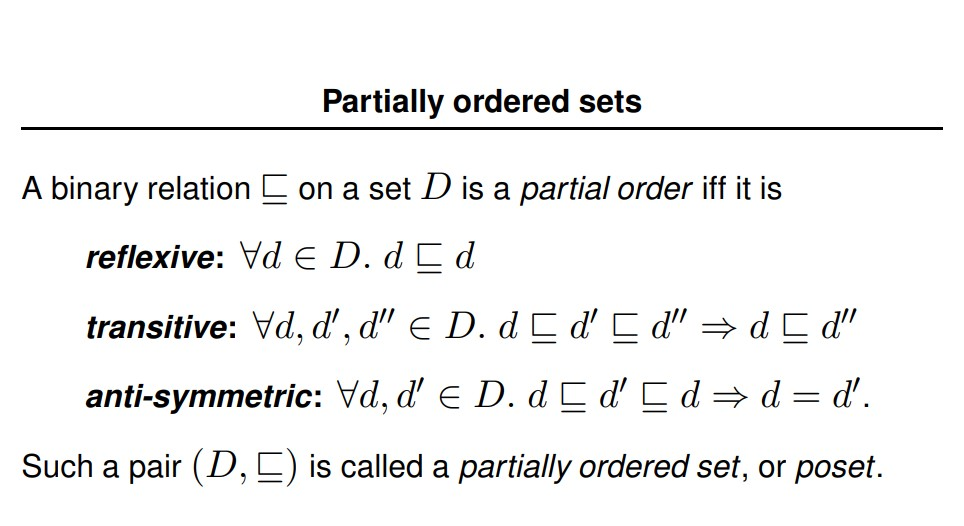
\includegraphics[scale = 0.7]{figs/poset_def}
\end{center}

The corresponding Agda code looks as follows:
\begin{minted}{agda}
record poset (D : Set) (_⊑_ : D → D → Set) : Set where
  field
    reflexive     : ∀ {d : D} → d ⊑ d 
    transitive    : ∀ {d d′ d″ : D} → (d ⊑ d′) → (d′ ⊑ d″) → (d ⊑ d″)
    antisymmetric : ∀ {d d′ : D} → (d ⊑ d′) → (d′ ⊑ d) → d ≡ d′
\end{minted}
This similarity was a key aim of my project. One of the main benefits of proof formalisation is that it massively narrows what one must trust (Cite/footnote talia ringer). To know that my Agda code is correct, one doesn't need to take it on faith, only that Agda's type-checker itself is correct. With that assumption, the code's correctness follows logically from the fact it type checks. However, this sounds very convenient, but it is very easy to prove things in Agda that are true, but not what you are trying to prove, or to be unable to prove things that are true. Therefore, to properly understand what it is that code is trying to prove and whether it succeeds, it is not only important that one's code type-checks, but also that it can be visibly seen to have type signatures corresponding to the intended theorems. 

For example, I may try to prove that all posets have a least element\footnote{This example is not a theorem. For example, the integers under the normal ordering relation do not have a least element.} and I may conceivably create a function in Agda whose type signature is:
\begin{minted}{agda}
poset-least-element : {P⊑ : poset P ⊑} → least-element P
\end{minted}
That is a function which takes a poset (with underlying set P and relation ⊑) and returns a least element of P. Since in Agda all functions terminate and are total, the function corresponding to this type signature (if it typchecks) is a proof that all posets have least elements.

But, the important point here has a symmetry with the point of denotational semantics. The map is not the territory (Footnote) and the \texttt{least-element} record defined in Agda may not accurately represent what a least element of a set really is. So, knowing that code type checks and thus that theorems' proofs are valid in Agda, is only good in so far as one trusts that the objects in question are encoded correctly. 

It was thus a key aim of my project to encode the objects not just correctly but obviously so, as far as possible: the closer to the course's definitions (both in content and notation), the more confident the reader can be that the \texttt{poset} in my code is the same as in the lectures and the wider study of posets. 

This is not as straightforward as it sounds however, as this task directly clashes with the process of formalisation. Often the representation chosen in lectures for ease of student understanding is not as easy to work with and may lead to later difficulties. Thus, while the following page (INCLUDE IMAGES) has comparisons of the course's definitions of objects and the straightforward way to try to mimic these, they are not actually (in all cases) the definitions I eventually settled on. 

To try to illustrate the range of ways of representing things, both in Agda, and mathematically, there will be two case studies, I will highlight both chains and posets, but note that for most objects, similar thoughts and issues arise. 
\subsubsection{Posets}
A poset is defined in the course\footnote{and everywhere else, this is a well-agreed-upon term. C.f. ``domain" or ``PCF" which differ in definition depending on author.} as a set, a relation on that set and some properties of that relation. Agda's basic syntax for defining novel types has two options. One can define a datatype with corresponding constructors (similar to ML-derived languages), or one can define records. Records are simply product types with named fields, each of which has its own type. 

It is not obvious what constructors for a poset would look like, or why there would be more than one of them. One choice would be simply the syntax \texttt{poset P $\leq$ reflexive transitive antisymmetric} where $P$ and $\leq$ are the relevant type and relation, and \texttt{reflexive}, \texttt{transitive} and \texttt{antisymmetric} are the relevant proofs. However with only a single constructor, this may as well be a record. 

But, even then, choices remain. Records are parameterised: that is, they may take inputs (via their type) that are not one of their fields. It is not always clear what belongs as a parameter, and what belongs as a field in a record. Thus, rather than the above definition, we could instead define analogously (footnote about Grothendieck universes):
\begin{minted}{agda}
record poset : Set where
  field
    A : Set
    R : A → A → Set
    reflexive     : ∀ {d : D} → d ⊑ d 
    transitive    : ∀ {d d′ d″ : D} → (d ⊑ d′) → (d′ ⊑ d″) → (d ⊑ d″)
    antisymmetric : ∀ {d d′ : D} → (d ⊑ d′) → (d′ ⊑ d) → d ≡ d′
\end{minted}

Or, we could instead say that a poset is a set with a partial order on that set. This could lead to:
\begin{minted}{agda}
record partial-order (A : Set) : Set where
  field
    R : A → A → Set
    reflexive     : ∀ {d : D} → d ⊑ d 
    transitive    : ∀ {d d′ d″ : D} → (d ⊑ d′) → (d′ ⊑ d″) → (d ⊑ d″)
    antisymmetric : ∀ {d d′ : D} → (d ⊑ d′) → (d′ ⊑ d) → d ≡ d′

record poset : Set where
  field
    A  : Set
    po : partial-order A
\end{minted}

These choices may seem relatively inconsequential, but indeed not only do such choices affect the ease of writing and reading the code that results, but they can make some ideas almost impossible to express (or relatively easy). Note for example, that in our first choice of implementing \texttt{poset} where the set and relation are parameters, there is no type of posets generally, and in fact all posets of the same type (i.e. sharing the same underlying set and relation) are essentially the same. 

Thus, if we wish to quantify over all posets, we need to first quantify over all sets, all corresponding relations, and then over all posets with the bound set variable, and bound relation variable. This approach does not seem too harmful at first, but quickly becomes almost insurmountable if one chooses to follow it. The interested reader is invited to (CITE OLD COMMIT) where one can see my code which originally took this approach. The theorems I wished to prove quickly became difficult to even provide the type signature for, let alone the actual proofs. For example, in an ideal world, to provide a type signature for a fixpoint operator that takes a function, and returns its least prefixed point, one might hope to write:
\begin{minted}{agda}
fixpoint : (A : Set) → (f : A → A) → continuous-function f → least-pre-fixed f
\end{minted}
or even just:
\begin{minted}{agda}
fixpoint : continuous-function → least-pre-fixed
\end{minted}
where the actual definition of $f$ (and hence its domain and codomain) is included in the record. 

However, if one needs to quantify over posets to do so, one might then need to quantify over the underlying sets of these posets (if they are parameters) and since a function has a domain and a codomain, this would require even more quantifying variables, and the type signature may become massively confused, to something like\footnote{This is a real example, with the name of the function changed}
\begin{minted}{agda}
fixpoint : (D : Set) (_⊑_ : D → D → Set) 
    (P : poset D _⊑_) (⊥ : D) (P′ : domain P ⊥) (f : D → D) 
    (cont-fun : continuous-fun P P f) 
  → least-pre-fixed P f
\end{minted}

This becomes unwieldy quickly. 
\subsubsection{Chains}
The difficulty of defining posets is mostly artificial, and introduced only by the attempt at formalisation. That is, to a mathematician, defining posets as a set with a partial order is not some wide and loose definition, but in fact narrow and restrictive. It is only the introduction of the mechanics of Agda that complicate things. This is not universally true though, some difficulties exist outside of Agda. The most obvious example is a chain (although in a more pathological programming language, real numbers would suffice well too see CITE). 

A chain \footnote{as typically presented, not as in the course} is a subset of a poset that is totally ordered. We can thus also view the ordered chain as an increasing sequence of values from a set. If we make the extra assumption that the subset is countable\footnote{It may seem odd to write off uncountable chains, but they are not so important in the real of finite computations}, then we can view a chain as a function from (a subset of) $\mathbb{N}$ to the poset. A mathematician can prove that these representations are isomorphic and thus not be too bothered about which is chosen, but for formalisation the implications matter. Even beyond that, we hit the issues of the previous section when it comes to how to encode in Agda the chosen representation. If we choose to represent a chain as a sequence, do we choose a lazy sequence, or a map from a subset of the naturals, or a map from all the naturals where sequences are just padded by their final element? 

Along with posets comes their basic structure-preserving maps: monotone functions (a function where $x \leq y$ implies $f x \leq f y$ (where $\leq$ is overloaded, and is standing in for two different relations on potentially two different sets)). Thus, a natural choice in my case dealing only with posets (and richer structures built on top of them) is to treat chains as monotone functions, from the naturals to a poset. This turns out to work, and indeed from my experience seems to work better than other choices, but it is certainly not obvious a priori whether that will be the case.

This a priori uncertainty, and necessity of immediately choosing an encoding, is one of the main difficulties of formalising some parts of mathematics. In much the same way that many linear algebra problems are simplified by avoiding a basis (footnote Senia shedyvasser quote), many problems are easer to reason about on pen and paper without specifying the encoding accompanying them. Noone who wishes to compute $\sqrt{2} + \sqrt{3}$ would want to first choose whether they were using the Cauchy-sequence representation or the Dedekind-cut based representation. 
\subsection{The ``nice" encodings and the actual interpretations}
With that said, the following figures show for the main objects of domain theory the definition in the lecture notes, the Agda definition that seems to correspond most closely to it, and the definition I eventually went with.
\subsection{Commentary}
\section{Domain theory theorems}
\subsection{Useful tools}
The early part of the course is full of results that seem to be demonstrations of how to use the definitions we have learnt, moreso than particularly useful theorems. However, some turn out to be critically important in later results. I here mention a couple, noting particularly a result that is later important, and a result that seems trivial but is difficult to prove. 
\subsubsection{Flat domains}
A flat domain is a domain constructed from a set, by adding one additional bottom element, and defining the relevant relation as equality (with the caveat that the bottom element is related to every other element). It is easy to check (\textit{with paper}) that this gives a valid domain: equality is an equivalence relation and so in particular a partial order; there is a bottom element; and chain-completeness is not a very interesting property here: all chains are either a constant element, or the bottom element and then a constant element.

However, it is precisely this ``boringness" of the chains that creates havoc. Agda and the programs one writes in it are normally constructive. To give a proof that $A$ implies $B$, one provides a function $A \to B$. It is not sufficient to prove that there is not a function from not $A$ to $B$ (this would be a classical proof by contradiction). Thus to prove that a domain is chain-complete, one must specify how, given a chain, one can compute its least upper bound. 

But, Agda also has a termination checker, and the problem of computing a lub of a chain in a flat domain is undecidable. The following argument is not rigourous but is instructive. Consider a chain that begins with a long (but finite) sequence of terms, each of which is the bottom element. To know whether the chain is only made up of the bottom element, or contains another element, one must keep checking further and further. No finite procedure is guaranteed to allow us to determine whether the chain is only the bottom element, or contains another element, and thus what the correct lub is. 

This problem may seem an artefact of the choice of representation of chains, but the problem is deeper than that. As De Jong mentions, one can prove that the flat (i.e. only equality-related) natural numbers forming a complete partial order (independent of representation of chains) implies something independent of Martin-Lof (UMLAUT) type theory and that is provably false in some constructive logics. This is a deep problem and tackled in myriad ways. De Jong uses a category-theoretic approach involving the so-called lifting monad ...


For my part, I use Agda's postulate feature, which allows us to define a usable function, only providing its type signature. However, this is not a silver bullet. While we can use this postulate, we can not prove much about anywhere we do use it, since it doesn't ``exist" per se, it just makes the type checker happy. 

The simplest postulate one could use to solve this problem would be simply to say that all chains in a flat domain have a lub. That is (where \texttt{flat-domain-pos} provides the poset of a flat domain, since chains are defined on posets, not domains):
\begin{minted}[fontsize = \small]{agda}
postulate chain-complete-flat-domain-pos-B : ∀ {B} 
  → (c : chain (flat-domain-pos B)) 
  → lub c
\end{minted}

However, the postulate I use (which implies the ``simpler" one) is:
\begin{minted}[fontsize = \small]{agda}
postulate flat-domain-chain-eventually-constant : ∀ {B} 
  → (c : chain (flat-domain-pos B)) 
  → eventually-constant c
\end{minted}
In this case, \texttt{eventually-constant c} is a record showing a given chain is eventually constant. It is defined as (where \texttt{g c m} is the $m$'th element of chain $c$, since \texttt{g c} is the underlying function of the chain):
\begin{minted}{agda}
record eventually-constant {P : poset} (c : chain P) : Set where
  field
    index : ℕ
    eventual-val : A P
    eventually-val : {m : ℕ} → index ≤ m → g c m ≡ eventual-val
\end{minted}
Note that in the constructive setting, we need to be able to access the index at which it becomes constant. This postulate is sufficient to show that flat posets are indeed chain-complete. To do this, we just need to create a \texttt{lub} record for any given chain. We define a function
\begin{minted}{agda}
chain-complete-flat-dom : {A : Set} → (c : chain (flat-domain-pos A)) → lub c
\end{minted}
A \texttt{lub} record has 3 fields: 
\begin{itemize}
\item The $\sqcup$ field states what element is the lub of a chain. For an eventually constant chain, this is the value the chain eventually takes on. We thus take the \texttt{eventual-val} field of the record our postulate gives us. 
\begin{minted}{agda}
⊔ (chain-complete-flat-dom c) 
= 
eventual-val (flat-domain-chain-eventually-constant c)
\end{minted}
\item The \texttt{lub1} field is a proof that every element in the chain is beneath the $\sqcup$ field. To do this, we perform a case analysis based on whether the index, $n$, of a given element in the chain is before or after the index after which the chain becomes constant, \texttt{index}. We do this using Agda's \texttt{with} feature, which allows us to perform a case-analysis based on an intermediate computation. In this case, we use a function \texttt{≤-dichotomy} which takes a pair of integers and returns a proof that one is less than or equal to the other. We call this on $n$, the index of the arbitrary element of the chain, and \texttt{index}, the index after which the chain becomes constant. 

In the first case, we use the monotonicity of the chain to show that the chain element is lower than the eventual val. In the second case, we use reflexivity of the poset\footnote{Technically, we use a separate lemma that looks like reflexivity, but rather than giving a proof of $a \leq a$ for all $a$, it takes a proof of $a \equiv b$ to construct a proof of $a \leq b$ (hence the name).}.

The arguments in braces are a nice feature of Agda's that has previously shown up, till now unremarked-upon. These are \textit{implict arguments}. When type checking, Agda performs unification to solve for these arguments if unspecified. This often enables less verbose code.
\begin{minted}[fontsize=\small]{agda}
lub1 (chain-complete-flat-dom {A} c) {n} 
    with ≤-dichotomy {n} {index (flat-domain-chain-eventually-constant c)}
...  | inj₁ n≤index = 
       a≤b≡c→a≤c′
         {B⊥ A} {R (flat-domain-pos A)}
         (mon c n≤index)
         (eventually-val (flat-domain-chain-eventually-constant c) (refl-≤))
...  | inj₂ index≤n = 
       a≡b→a≤b
         {flat-domain-pos A}
         (eventually-val (flat-domain-chain-eventually-constant c) index≤n)
\end{minted}
\item
The \texttt{lub2} field is a proof that $\sqcup$ is a least upper bound, not just an upper bound (which \texttt{lub1} shows). Specifically, it takes a proof that some other element \texttt{d′} is an upper bound (this proof is labelled \texttt{x}), and constructs a proof that the $\sqcup$ field is less than or equal to \texttt{d′}.

Our proof shows that the $\sqcup$ field is equal to \texttt{g c (index (flat-domain-chain-eventually-constant c))}, i.e. the \texttt{index}'th element of the chain. It then applies the hypothesis \texttt{x} (that \texttt{d′} is an upper bound) and a kind of transitivity\footnote{Here we use a function that takes a proof that $a \equiv b$ and a proof that $b \leq c$ and returns a proof that $a \leq c$.} to conclude that $\sqcup$ is below \texttt{d′} as required. 
\begin{minted}{agda}
lub2 (chain-complete-flat-dom {A} c) {d′} x = a≡b≤c→a≤c
  {B⊥ A}
  {R (flat-domain-pos A)}
  {eventual-val (flat-domain-chain-eventually-constant c)}
  {g c (index (flat-domain-chain-eventually-constant c))} {d′}
  (Eq.sym (eventually-val (flat-domain-chain-eventually-constant c) refl-≤))
  x
\end{minted}
\end{itemize}
\subsubsection{The diagonalising lemma}
Frequently one ends up nesting lubs (when). From calculus, one may recall with frustration that the conditions around when limits commute are highly technical and detailed. However, we deal only with ``nice" functions, in particular monotone functions, and this suffices to prove that in all cases:
\begin{equation} \label{comm-double-lub}
\bigsqcup_{m \geq 0} \left( \bigsqcup_{n \geq 0} d_{m, n}\right) = 	\bigsqcup_{n \geq 0} \left( \bigsqcup_{m \geq 0} d_{m, n}\right).
\end{equation}
While this is an interesting result, its much more useful form is that both side of this equation are equal to a single lub, over the diagonal chain:
\begin{equation} \label{diag}
\bigsqcup_{k \geq 0} d_{k, k}.
\end{equation}
This enables us to simplify calculations, using continuous functions to push two lubs together and then using this result to transform it into a single lub. This is a common proof technique and comes up when proving the continuity of the evaluation function, the if-operator, and the fixpoint operator. 

This is a result that plays nicely with Agda, insofar as formalising its proof requires little advanced machinery or creativity, relative to writing it down with pen-and-paper. We define three diagonalising lemmas:
\begin{minted}{agda}
diagonalising-lemma-1 : (P : domain) 
  → (double-index-fun : monotone-fun nats²-pos (pos P))
  → ⊔ ((chain-complete P) (chain-⊔fₙₖ-with-n-fixed P double-index-fun)) 
     ≡ 
     ⊔ ((chain-complete P) (fₖₖ-chain P double-index-fun))

diagonalising-lemma-2 : (P : domain) 
  → (double-index-fun : monotone-fun nats²-pos (pos P))
  → ⊔ ((chain-complete P) (chain-⊔fₖₙ-with-n-fixed P double-index-fun)) 
     ≡ 
     ⊔ ((chain-complete P) (fₖₖ-chain P double-index-fun))

diagonalising-lemma : (P : domain) 
  → (double-index-fun : monotone-fun nats²-pos (pos P))
  → ⊔ ((chain-complete P) (chain-⊔fₙₖ-with-n-fixed P double-index-fun)) 
     ≡ 
     ⊔ ((chain-complete P) (chain-⊔fₖₙ-with-n-fixed P double-index-fun))
\end{minted}
In the above, the last result corresponds to equation \ref{comm-double-lub} while the first two results are the two equalities with \ref{diag}. If we can show the first two results, the final one follows easily via transitivity of equality:
\begin{minted}{agda}
diagonalising-lemma P double-index-fun = Eq.trans 
  (diagonalising-lemma-1 P double-index-fun) 
  (Eq.sym (diagonalising-lemma-2 P double-index-fun))
\end{minted}
We use \texttt{Eq.sym} to turn a proof that $a\equiv b$ to a proof that $b \equiv a$. Thus, the meat of the problem is providing the function body for \texttt{diagonalising-lemma-1} and \texttt{diagonalising-lemma-2}. Each is not hard to prove, but neither is trivial. We present and explain here only the proof of \texttt{diagonalising-lemma-2}: this corresponds to
\[
\bigsqcup_{m\geq 0} \left( \bigsqcup_{n\geq 0} d_{m,n} \right) = \bigsqcup_{k \geq 0} d_{k, k}.
\]
Our proof goes by antisymmetry of the underlying partial order. We thus need to show that
\begin{equation} \label{anti-sym1}
\bigsqcup_{m \geq 0} \left( \bigsqcup_{n\geq 0} d_{m,n} \right) \leq \bigsqcup_{k \geq 0} d_{k, k}
\end{equation}
and
\begin{equation} \label{anti-sym2}
\bigsqcup_{k \geq 0} d_{k, k} \leq \bigsqcup_{m \geq 0} \left( \bigsqcup_{n\geq 0} d_{m,n} \right) .
\end{equation}
We first tackle \ref{anti-sym1} using the universal property of lubs, (aka \texttt{lub2}) which states that a least upper bound is less than or equal to any other upper bound. So it suffices to show that 
\[
\bigsqcup_{k \geq 0} d_{k, k} 
\]
is an upper bound, that is
\[
\forall m \geq 0. \left( \bigsqcup_{n\geq 0} d_{m,n} \right) \leq \bigsqcup_{k \geq 0} d_{k, k}.
\]
We take an arbitrary $m$, and then again we wish to show that a lub is less than something else. We thus use \texttt{lub2} again, so it suffices to show that
\[
\forall n \geq 0. d_{m, n} \leq \bigsqcup_{k \geq 0} d_{k , k}.
\]
We do this using a lemma that shows transitively that $d_{m,n} \leq d_{\text{max}(m,n), \text{max}(m,n)} \leq \sqcup d_{k,k}$ where the first inequality is by monotonicity and the final inequality is shown using the property \texttt{lub1}. 

Our work is not done (and hopefully now we are starting to see the annoyance of being explicit about every detail mathematically), as we need to show the other half of the antisymmetry, inequality \ref{anti-sym2}. This however is easier. We can use \texttt{lub2} again, so we really only need to show that
\[
\forall k \geq 0.s d_{k,k} \leq \bigsqcup_{m \geq 0} \left( \bigsqcup_{n\geq 0} d_{m,n} \right).
\]
We do this by transitivity. We show $d_{k,k} \leq \sqcup_{m \geq 0} d_{m,k} \leq \sqcup \sqcup d_{m,n}$ where both inequalities hold by straightforward applications of \texttt{lub1}. That was a frustatingly long and verbose proof in words, in comparison to a few lines in the course notes (CITE). In addition, even that description is not sufficient to account for all the code\footnote{This verbosity is one reason some may find Agda's lack of tactics unsatisfying. Other Curry--Howard based proof-assistants support writing simpler code that expands to longer code using tactics, however it is often much harder to parse for a reader, although shorter.}, since the code relies upon a few functions\footnote{Namely, \texttt{chain-⊔fₖₙ-with-n-fixed} and \texttt{chain-fₘₙ-with-n-fixed}.} that are not explained; proofs that the chains involved in the manipulations are valid chains. 

The corresponding Agda code is:
\begin{minted}{agda}
diagonalising-lemma-2 P double-index-fun = let ⋃ = chain-complete P in
  antisymmetric (pos P)
    (lub2
      (⋃ (chain-⊔fₖₙ-with-n-fixed P double-index-fun))
      (λ {m} →
        lub2
          (⋃ (chain-fₘₙ-with-n-fixed P double-index-fun m))
          (λ {n} → dₘₙ≤⊔dₖₖ P double-index-fun)))
    (lub2
      (⋃ (fₖₖ-chain P double-index-fun))
      (λ {n} →
        transitive (pos P)
          (lub1 (⋃ (chain-fₘₙ-with-n-fixed P double-index-fun n)) {n})
          (lub1 (⋃ (chain-⊔fₖₙ-with-n-fixed P double-index-fun)))))
\end{minted}
\subsection{Continuous functions}
A large amount (how much?) of the code written proves that certain functions are continuous. A simpler denotational semantics, where types correspond to sets, and functions in code merely to mathematical functions avoids almost all of this trouble. However, this is the price we pay for being able to work with fixed points and partial functions properly. (CITE SCOTT QUOTE).
\subsubsection{Continuity of the if-operator}
Our approach to proving the if-operator is continuous is arduous. This is perhaps the best example of a recurring theme in formalising proofs (CITE), that much of the work is in spelling out details and being careful with minor points that humans bother little about. In the notes for the course, there is a proposition that the function is continuous, and following that there is a lemma that functions of two arguments are continuous iff they are continuous in each argument (with the other fixed). This is all that is mentioned which is terse and leaves the underlying point (that we can prove if is continuous, by showing it is continuous in each argument) unsaid, but understandable.

Nonetheless, the file \texttt{if-cont.agda} is around 600 lines, involving some detailed equational reasoning, as well as proofs of the above lemma, and proofs that if is indeed continuous in each argument, and that every chain in the intermediate reasoning is a valid chain. 

The final proof of its continuity is:
\begin{minted}{agda}
if-cont : ∀ {D} → cont-fun (domain-product 𝔹⊥ (domain-product D D)) D
if-cont {D} =
  slide-33-prop-cont
    {𝔹⊥} {domain-product D D} {D}
    if-g
    (if-mon-first {D}) 
    (λ {d} {e₁} {e₂} → if-mon-second D d e₁ e₂)
    if-cont-first
    (if-cont-second {D})
\end{minted}
The \texttt{slide-33-prop-cont} function takes a function of two arguments, proofs of its monotonicity in each, and proofs of its continuity in each to produce a continuous function (with a proof of its continuity). I will avoid the tedious details but the curious reader is invited to (CITE).

Of particular interest is how proving continuity in the first argument involves chains on flat domains. This requires\footnote{somewhat, arguably we just push the problem to determining the eventual value of a chain, which is still non-constructive, but is at least workable with for proving equalities.} a constructive proof of showing chains on flat domains do have lubs. Without it, we can't prove equality between this lub and something else, if the lub doesn't actually exist constructively. 

The definition of \texttt{if-g} and the proofs of monotonicity in its first and second arguments are fairly easy, so we show them here:
\begin{minted}{agda}
if-g : ∀ {D} → A (pos (domain-product 𝔹⊥ (domain-product D D))) → A (pos D)
if-g {D} x with (x fzero)
...                     | inj false = x (fsucc fzero) (fsucc fzero)
...                     | inj true  = x (fsucc fzero) fzero
...                     | ⊥₁        = least-element.⊥ (bottom D)
\end{minted}
We define \texttt{if-g} by case-analysis on its first argument\footnote{\texttt{x} is a dependent product from a finite subset of the naturals, so \texttt{x} fzero just returns the first part of \texttt{x}.}. If false, then we take the second part of the second part of \texttt{if-g}'s argument, if true then the first of the second, and if bottom, then we return the bottom element of the appropriate domain. 
\begin{minted}{agda}
if-mon-first : (D : domain)
  → ((b b′ : B⊥ Bool)
  → (e : A (pos (domain-product D D)))
  → (R (pos 𝔹⊥)) b b′
  → (R (pos D)) (if-g {D} (pair b e)) (if-g {D} (pair b′ e)))

if-mon-first {D} z≼n = least-element.⊥-is-bottom (bottom D)
if-mon-first {D} x≼x = reflexive (pos D)
\end{minted}
We pattern-match on the proof that \texttt{b} and \texttt{b′} are related. Since the domain is flat, we have two cases. The first case is that one is the bottom element, and so to show it is monotonic, we just need to show that the bottom of \texttt{D} is below \texttt{if-g {D} (pair b′ e)}, but the bottom of $D$ is below everything in \texttt{D} so this follows easily.

The second case is that \texttt{b} and \texttt{b′} are the same element, in which case so too are the output of \texttt{if-g {D} (pair b e)} and \texttt{if-g {D} (pair b′ e)}, so we can use reflexivity of relation in \texttt{D}. 
\begin{minted}{agda}
if-mon-second : (D : domain)
  → ((b : B⊥ Bool)
  → (e e′ : A (pos (domain-product D D)))
  → (R (pos (domain-product D D))) e e′
  → (R (pos D)) (if-g {D} (pair b e)) (if-g {D} (pair b e′)))
if-mon-second D ⊥₁ e e′ e≤e′ = ⊥-is-bottom (bottom D)
if-mon-second D (inj false) e e′ e≤e′ = e≤e′ (fsucc fzero) 
if-mon-second D (inj true) e e′ e≤e′ = e≤e′ fzero
\end{minted}
Our second argument is itself a pair and a pair being below another pair means each part is. So if we have \texttt{e ≤ e′} or more accurately \texttt{(R (pos (domain-product D D))) e e′} we thus have that the first part of \texttt{e} is below the first part of \texttt{e′} and that the second part is too. So we case match on the boolean value. If it is $\bot$, then we are in the simple case, and if it is false, then we project out the second half of our proof that $e \leq e′$, and the first half if true. 
\subsubsection{Continuity of the fixpoint-operator (and Tarski's fixed point theorem)}
The crowning jewel of domain theory for the purposes of PCF-encoding is this theorem: that all continuous functions have a least fixed point, moreoever that it is given by
\[
\bigsqcup_{n \geq 0} f^n(\bot)
\]
and moreover again that the function \texttt{fix} which given a continuous $f$ returns the least fixed point of $f$, is itself a continuous function\footnote{Tarski's fixed point theorem is that the fix operator exists and supplies the least pre-fixed-point, and that it is a fixed point, but not that the operator is continuous itself}.
\section{PCF and its properties}
As specified earlier, Scott's original definition of PCF is not quite what is chosen here. Namely Scott avoided lambdas, although he viewed it as the ``proper thing" to introduce them, as he didn't ``want to formulate all the rules about free and bound variables". This is a common theme in formalising programming languages, that lambdas are a pain-point, despite the rules around free variables being simple to state and fairly intuitive. 

Namely we make two principle alterations: firstly, we make all the alterations of the course (including lambdas and thus avoiding the S and K combinators) and one additional very small change. Namely we make zero its own predecessor, where the course (and Scott's original work) make it undefined. This has a few effects. For one thing, it allows the language to have progress (if one chooses the course's definitions, every well typed non-value term reduces (not necessarily to a normal form!) apart from \texttt{pred(0)}). Furthermore, it changes the predecessor function from not having any obvious fixed points (other than the undefined bottom element) to having zero as a fixed point.
\subsection{Intrinsic typing} 
Basically copy what Ted and Wadler said I guess?
\subsection{Operational Semantics and Progress (and preservation for free)}
\subsubsection{Operational Semantics}
We define a small-step operational semantics. Note that this is different from the big-step operational semantics presented in the lecture notes, but I claim my definition is equivalent. There are very few surprises, other than the changing of \texttt{pred(zero)} from the course, and everything more or less works nicely, apart from having to deal with substitution for the lambdas. (maybe present a proof that the same evaluation rules hold?). 

We evaluate the left side of applications first:
\begin{minted}{agda}
data _—→_ : ∀ {Γ A} → (Γ ⊢ A) → (Γ ⊢ A) → Set where

  ξ-·₁ : ∀ {Γ A B} {L L′ : Γ ⊢ A ⇒ B} {M : Γ ⊢ A}
    → L —→ L′
    → L · M —→ L′ · M
\end{minted}
We evaluate arguments to \texttt{pred}, \texttt{suc}, if-clauses and \texttt{is-zero} where possible:
\begin{minted}{agda}
  ξ-suc : ∀ {Γ} {M M′ : Γ ⊢ `ℕ}
    → M —→ M′
    → `suc M —→ `suc M′

  ξ-pred : ∀ {Γ} {M M′ : Γ ⊢ `ℕ}
    → M —→ M′
    → `pred M —→ `pred M′
  
  ξ-if : ∀ {Γ A} {B B′ : Γ ⊢ `bool} {x y : Γ ⊢ A}
    → B —→ B′
    → if B then x else y —→ if B′ then x else y

  ξ-is-zero : ∀ {Γ} {M M′ : Γ ⊢ `ℕ}
    → M —→ M′
    → `is-zero M —→ `is-zero M′
\end{minted}
We have the expected $\beta$-reductions for if-clauses:
\begin{minted}{agda}
  β-if₁ : ∀ {Γ A} {x y : Γ ⊢ A}
    → if `true then x else y —→ x

  β-if₂ : ∀ {Γ A} {x y : Γ ⊢ A}
    → if `false then x else y —→ y
\end{minted}
Again, we have normal reductions for \texttt{pred} and \texttt{is-zero}. These $\beta$ rules only apply when the relevant other terms are fully evaluated. They thus require a proof of the relevant term being a value to be used. We do not need a reduction rule for \texttt{`suc M} where \texttt{M} is a value. This is because these are normal forms; there is no other \texttt{Value} representation of 1, other than \texttt{`suc `zero}. Note here also that we include \texttt{β-pred₁}: this is the departure from the course and Scott's version of PCF. 
\begin{minted}{agda}
  β-pred₁ : ∀ {Γ : Context}
    → `pred (`zero) —→ `zero {Γ}

  β-pred₂ : ∀ {Γ : Context} {M : Γ ⊢ `ℕ}
    → Value M
    → `pred (`suc M) —→ M

  β-is-zero₁ : ∀ {Γ}
    → `is-zero `zero —→ `true {Γ}

  β-is-zero₂ : ∀ {Γ} {M : Γ ⊢ `ℕ}
    → Value M
    → `is-zero (`suc M) —→ `false 
\end{minted}
Our most interesting two reduction rules are lambdas and the fix-operator. 

We say that $\lambda N \cdot W$ steps to $N [W]$ where $[W]$\footnote{This is a separate function, that requires some care to define correctly. Wadler covers the details in CITE.} means that $W$ is substituted for the innermost de Bruijn index (i.e. this is the de Bruijn way of saying $(\lambda x. N) W \to N[W/x]$). This is therefore call-by-name evaluation, where the argument is not reduced before substitution. This is crucial for allowing the fix point operator to work correctly (why?). 
\begin{minted}{agda}
  β-ƛ : ∀ {Γ A B} {N : Γ , A ⊢ B} {W : Γ ⊢ A}
    → (ƛ N) · W —→ N [ W ]
\end{minted}
Additionally, since we are using small step semantics, the definition of fix of an endofunction (note the type signature!) is quite simple:
\begin{minted}{agda}
  β-μ : ∀ {Γ A} {N : Γ ⊢ A ⇒ A}
    → μ N —→ N · (μ N)
\end{minted}
\subsection{Denotational Semantics}
We have three denotation functions, namely those which map a type (in PCF) to a domain, a context (in PCF) to a domain, and those which map terms of type $\tau$ under assumptions $\Gamma$ to continuous functions from $\llbracket \Gamma \rrbracket$ to $\llbracket \tau \rrbracket$. The denotation of ground types is what you would expect, namely the flat domain. We use the underlying booleans and naturals from Agda and augment them with the flat ordering and extra bottom element. 

For the denotation of a function-space, we take a function domain. That a function-space between two domains can be ordered to form a domain is a useful result (Where is this proved in the course?), proved in the definition of \texttt{function-domain}. Because this typechecks, we know that \texttt{function-domain} is a valid domain (due to the type signature of the function), and thus that it has a least element, and a partial order, and is chain-complete (indeed these are all provided explicitly in CITE). 
\begin{minted}{agda}
⟦_⟧ : Type → domain
⟦ `ℕ ⟧ = ℕ⊥
⟦ `bool ⟧ = 𝔹⊥
⟦ τ ⇒ τ′ ⟧ = function-domain ⟦ τ ⟧ ⟦ τ′ ⟧
\end{minted}
We then define contexts as the depedent product domain. INSERT STUFF ABOUT CARTESIAN N-ary products vs binary products iterated?
\begin{minted}{agda}
context-⟦_⟧ : Context → domain
context-⟦ Γ ⟧ = domain-dependent-product (Fin (length Γ)) (λ x → ⟦ lookup₂ {Γ} x ⟧)
\end{minted}
We then turn to the denotations of well-typed terms (these are the only terms due to intrinsic typing). While the course separates the denotations from the proofs that these are valid continuous functions, Agda saves us some time. Since we define denotations as continuous functions, Agda will only type check if we supply something that is proven continuous. Our type signature is:
\begin{minted}{agda}
⟦_⊢′_⟧ : ∀ {A} → (Γ : Context) → (M : Γ ⊢ A) → cont-fun context-⟦ Γ ⟧ ⟦ A ⟧
\end{minted}

Since our denotation is compositional (i.e. the denotation of an expression is a composition of the denotations of the subexpressions) a key lemma that we will use for all non-normal forms, is that the composition of two continuous functions is itself continuous. This has a somewhat lengthy proof in Agda (as we need to be explicit about not only the function, but the proof that it is continuous) but is not particularly troublesome. We present here its type signature. The curious reader is invited to look closer at CITE.
\begin{minted}{agda}
_∘_ : ∀ {D₁ D₂ D₃} → cont-fun D₂ D₃ → cont-fun D₁ D₂ → cont-fun D₁ D₃
\end{minted}

We then show constant functions are continuous\footnote{We call the lemma that this produces a continuous function \texttt{constant-fun}.}, and thus the denotations of zero, true and false are dealt with. 
\begin{minted}{agda}
⟦ Γ ⊢′ `zero ⟧ = constant-fun {Γ} ℕ 0
⟦ Γ ⊢′ `true ⟧ = constant-fun {Γ} Bool true
⟦ Γ ⊢′ `false ⟧ = constant-fun {Γ} Bool false
\end{minted}
We then show that extending a partial function to a flat domain in the obvious way (WHAT DOES THIS MEAN) gives us a continuous function. This takes care of the test-for-zero, the successor function, and the predecessor function, when combined with the recursing on their arguments. 
\begin{minted}{agda}
⟦ Γ ⊢′ `is-zero N ⟧ = z⊥ ∘ ⟦ Γ ⊢′ N ⟧
⟦ Γ ⊢′ `suc N ⟧ = s⊥ ∘ ⟦ Γ ⊢′ N ⟧
⟦ Γ ⊢′ `pred N ⟧ = p⊥ ∘ ⟦ Γ ⊢′ N ⟧
\end{minted}
This leaves us with exactly 5 cases: we show application is a continuous function in \texttt{ev-cont.agda}, we show the \texttt{if then else} function is continuous in \texttt{if-cont.agda}, we show the fixpoint operator is continuous in \texttt{fix-cont.agda} and we show that currying gives a continuous function in \texttt{cur-cont.agda}\footnote{For technical reasons, we use a helpful lemma here that essentially helps us convince Agda that our proof is valid. It takes a continuous function from a given context, and returns a continuous function from the product of the head of its context and its last element. The reason this matters is due to the subtle distinction between iterated binary products and general $n$-ary products.}.
\begin{minted}{agda}
⟦ Γ ⊢′ M₁ · M₂ ⟧ = ev-cont ∘ (pair-f ⟦ Γ ⊢′ M₁ ⟧ ⟦ Γ ⊢′ M₂ ⟧) 
⟦ Γ ⊢′ if M₁ then M₂ else M₃ ⟧ = if-cont ∘ (pair-f ⟦ Γ ⊢′ M₁ ⟧ (pair-f ⟦ Γ ⊢′ M₂ ⟧ ⟦ Γ ⊢′ M₃ ⟧))
⟦ Γ ⊢′ μ M ⟧ = tarski-continuous ∘ ⟦ Γ ⊢′ M ⟧ 
⟦ Γ ⊢′ ƛ_ {A = A} {B} M ⟧ = cur-cont (helpful-lemma-blah {Γ} {A} {B} ⟦ Γ , A ⊢′ M ⟧)
\end{minted}
Our one remaining case is the case of variables, but the denotation of a variable from a context containing it is just a projection function. 
\begin{minted}{agda}
⟦ Γ ⊢′ ` x ⟧ = project-x Γ x
\end{minted}
We use the intermediary function \texttt{project-x} which does a projection of a domain from a dependent product of domains, using a lemma that a certain equality holds. Again the details are not particularly interesting: these are the kinds of troubles introduced artificially. The lemma here is not something one would necessarily write on paper, but just a way of propogating information from the author to Agda's type checker. 
\subsection{Soundness}
As with most things to do with programming languages, the majority of the proof of soundness is an uninteresting and straightforward use of induction. The cases for most terms look like:
\begin{minted}{agda}
soundness (ξ-·₁ {L = L} {L′} {M} L→L′) =
  begin
    term-⟦ L · M ⟧
  ≡⟨ refl ⟩
    ev-cont ∘ pair-f term-⟦ L ⟧ term-⟦ M ⟧
  ≡⟨ cong (_∘_ ev-cont) (cong (λ x → pair-f x term-⟦ M ⟧) (soundness L→L′)) ⟩
    ev-cont ∘ pair-f term-⟦ L′ ⟧ term-⟦ M ⟧
  ≡⟨ refl ⟩
    term-⟦ L′ · M ⟧
  ∎
\end{minted}
Here, Agda is able to propogate our definition of the denotation of the term (hence the proof justification being \texttt{refl}, that is Agda can tell these two terms are the same), and then using the induction hypothesis (that the reduction of L to L' is sound and thus that the two denotations are the same) we can go from the second line to the third and then we are done. 

The interesting cases are those without induction hypotheses (correspondingly the ones that don't involve recursion in Agda). Of these, there are two classes: the slightly tedious (the cases for \texttt{if true then x else y} and \texttt{if false then x else y} require lemmas that are simple to prove but annoying to state) and the genuinely interesting cases: these are lambda abstractions and the case of the fix operator. This exactly mirrors the claim of the lecture course, in which these two cases are given, and the others are left unsaid. 
\subsubsection{The case of fix}
The fix operator case transforms relatively easily. The course notes say:
\begin{center}
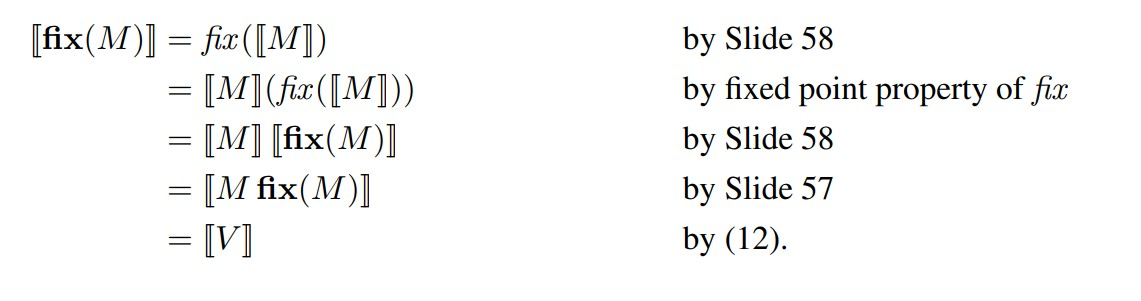
\includegraphics[scale = 0.7]{figs/fix_soundness}
\end{center}
and our code\footnote{Again, this has been manufactured to look similar to the lecture notes, this may disguise various difficulties coercing Agda to play nicely, but proving it did not require any extra mathematical insight, only familiarity with Agda.} mirrors this nicely:
\begin{minted}{agda}
soundness {A} (β-μ {N = N}) =
   begin
     term-⟦ μ M ⟧
   ≡⟨ refl ⟩
     tarski-continuous ∘ term-⟦ M ⟧
   ≡⟨ cont-fun-extensionality
     (λ x → lfp-is-fixed { ⟦ A ⟧ } {g (mon term-⟦ M ⟧) x })
    ⟩
     ev-cont ∘ pair-f term-⟦ M ⟧ (tarski-continuous ∘ term-⟦ M ⟧)
   ≡⟨ refl ⟩
     ev-cont ∘ (pair-f term-⟦ M ⟧ term-⟦ μ M ⟧)
   ≡⟨ refl ⟩
     term-⟦ M · (μ M) ⟧
   ∎
\end{minted}
Note that because we use small-step operational semantics, we prove that the denotation of (μ M) is identical of what it reduces to in one step: M · (μ M). The course notes instead have the hypothesis supplied by their big step semantics to justify a final line that equates these to whatever value they reduce to. 

It should also be noted that often in these cases we are trying to prove the equality of two functions, which means we need to use the extensionality postulate mentioned earlier. 
\subsubsection{The case of lambdas}

\chapter{Evaluation}

\chapter{Conclusions}

\end{document}